\chapter{The OpenRobots Ontology framework}
\label{chapt|oroserver}

This chapter introduces the \emph{OpenRobots Ontology} server and its
common-sense knowledge base.

We present a \textbf{functional description} of oro-server, and detail at
lenght its knowledge model. Its actual implementation is discussed in the next
chapter.

We also present in depth the \emph{OpenRobots Common-Sense Ontology} that
contains most of the knowledge at hand when the robot starts.

\section{Functional overview}
\label{sect|functional-overview}


We have adopted a centralized approach for knowledge management called
ORO~\cite{Lemaignan2010}. The platform is designed as a central
knowledge storage service implemented as a server where the robot
components can add or query statements at run-time. Figure~\ref{fig|oro-overview}
illustrates the main functional components of ORO.

\begin{figure}
\centering
  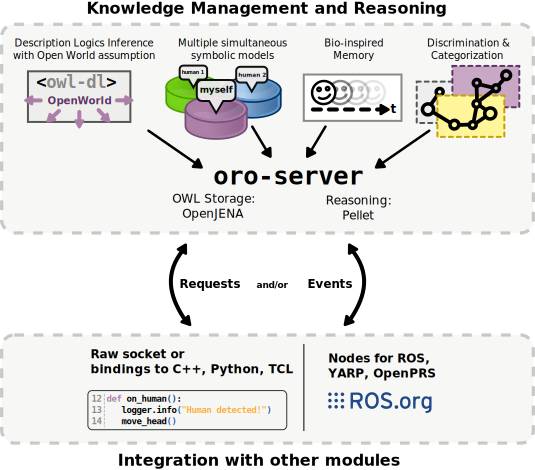
\includegraphics[width=0.8\linewidth]{oroserver/oro_architecture_functional.pdf}
  \caption{Overview of the ORO architecture.}
  \label{fig|oro-overview}
\end{figure}

At the core, ORO is build around the
OpenJena\footnote{\url{http://www.openjena.org}} ontology management library,
connected to the Pellet\footnote{\url{http://clarkparsia.com/pellet}}
reasoner.

A front-end accepts and manages connections to clients. The clients' requests
are processed by a set of internal modules: basic operations on statements,
but also higher cognitive and human-robot interaction related functionalities
are available. External plugins can also be easily added.

Besides acting as a facts database, the ORO platform exposes several
functions: operations on knowledge statements relying on inference (through a
continuous first-order logic classification process), management of
\emph{per-agent} symbolic models, and also higher cognitive and human-robot
interaction related functionalities like categorization of sets of concepts
or profiles of memory (that enable the robot to ``forget'' about some facts).

ORO also provides an event mechanism that allows components to be triggered
when specific events occur. A component can for instance subscribe to events
of kind \setstmt{?agent isVisible true, ?agent type Human}. As soon as the
perception layer detects a human in the robot's field of view and accordingly
updates the knowledge base, the executive layer is triggered. The event
framework also takes advantage of the inference capabilities of ORO. Thus an
event can be indirectly triggered if its triggering conditions can be
inferred to be true.



%%%%%%%%%%%%%%%%%%%%%%%%%%%%%%%%%%%%%%%%%%%%%%%%%%%%%%%%%%%%%%%%%%%%%%%%%%%%%%%
%%%%%%%%%%%%%%%%%%%%%%%%%%%%%%%%%%%%%%%%%%%%%%%%%%%%%%%%%%%%%%%%%%%%%%%%%%%%%%%

\section{The ORO Knowledge model}
\label{sect|knowledge-model}

\subsection{Expressiveness}

Unlike systems relying on logic programming like {\sc KnowRob}, ORO is purely
based on Description Logics: the ORO knowledge model is based on RDF triples
(\ie exclusively binary predicates). Triples \stmt{subject predicate object}
are the atoms of knowledge for ORO.

\paragraph{Reification} Since RDF triples constraint to binary predicates,
\emph{reification} is often required to express $n$-ary relations. For
instance, the relation \emph{A gives object B to C} can not directly be
represented in RDF. This relation is reified as \{\stmt{act1 type Action},
\stmt{act1 performedBy A}, \stmt{act1 actsOn B}, \stmt{act1 receivedBy C}\}. As
long as the instance \concept{act1} exists in the knowledge base, the orignial
relation \emph{A gives object B to C} is considered to hold. This kind of
reification is common in the ORO knowledge model.

Reification can also take place at a meta-level (this is the level usually
intended when knowledge manipulation API mention reification): a triple
\stmt{subject predicate object} can be itself reified in \{\stmt{stmt1 type
Statement}, \stmt{stmt1 hasSubject subject}, \stmt{stmt1 hasPredicate
predicate}, \stmt{stmt1 hasObject object}\}. This level of reification allows
to characterise to knowledge atoms themselves, for instance to specify when the
atom was added. The section on memory management in ORO server, below, gives
examples of usage of this meta-cognition feature.

Note that in traditional logical programming like Prolog, reification is rarely
strictly required since no constraints hold on the arity of predicates. To
store the date of creation of a facts, one could simply add it as a
supplementary argument of the predicate\footnote{In the case of time
representation, however, reification --- or, in the case of logic programming,
second order logic --- is commonly found through the \emph{fluents} mechanisms,
see section~\ref{sect|time-representation}}.

\paragraph{Open World Assumption}

%%%%%%%%%%
\subsection{How things are represented?}

\subsubsection{Role Representations}
Spatio-Temporal Representations:

\paragraph{Representation of space}
\paragraph{Representation of events and actions}

\subsubsection{Context modeling}
\subsubsection{Possible-Worlds and representing what others know}

\paragraph{Multi-model representation for Persepective-taking}
\label{sect|alterite}

...

We present at section~\ref{sect|perspectivetaking},
page~\pageref{sect|perspectivetaking} an 3D real-time environment, SPARK, that
allows to compute on-line several perspective aware symbolic properties.

\subsubsection{False beliefs and Theory Of Mind}
\label{sect|theory-of-mind}



\subsubsection{Introspection: Who am I? What can I do?}

\subsubsection{Multi-lingual support}
\label{sect|multilingual}

The RDF specification supports internationalisation by the way of
\emph{language tags}: plain literals may have an optional language tag (taken
from the standard RFC-3066) that tells in which human language the literal is
expressed.

ORO benefits from this mechanism, and can be configured to use a specific
language as default. When an language is explicitely selected, the translated
labels of concepts (when available in the underlying ontology) are used instead
of the default English ones. Section~\ref{sect|commonsense-i13n} gives more
details on the current level of internationalisation of the ORO common-sense
ontology.

Since only the labels (\ie the human-friendly name of the concepts) are subject
to translation, changing the default language of the ORO server has no semantic
impact: entities in the ontology always refer to same concepts. Same inferences
are drawn, same connections to knowledge sources are made, etc. The strenght of
semantic approaches is here well illustrated.

%%%%%%%%%%
\subsection{Reasoning Techniques}

Some of the main algorithms are presented here as well (like the algorithms for
classification and discrimination,~\ref{sect|discrimination}).


\subsubsection{Standard reasoning techniques}


Knowledge is stored as OWL/RDF ontologies in ORO. We use the Pellet reasoner to
classify them. This enables several type of reasoning:

\begin{itemize}
	\item reasoning on inheritance relations (\eg \emph{all bottles are containers}),
	\item property axioms
		\begin{itemize}
		\item entailments based on predicates' domain and range,
		\item cardinality constraints (including \concept{allValue}, 
		\concept{someValue}, \concept{hasValue}),
		\item property characteristics (symmetry, transitivity)
		\end{itemize}
	\item class restrictions like: \par \footnotesize \concept{Bottle} $\equiv$
		\concept{Artifact} {\bf that} (\concept{hasShape} {\bf value}
		\concept{cylinderShape})\footnote{This example uses the \emph{Manchester
		syntax}, \url{http://www.w3.org/TR/owl2-manchester-syntax/}} \normalsize
	\item set operations like: \par \footnotesize \concept{Color} $\equiv$ {\bf unionOf}(\concept{blue},
		\concept{green}, \concept{orange}, \concept{black}...) \normalsize
	\item generic SWRL ({\em Semantic Web Rule Language}) rules like: \par
		\footnotesize \concept{looksAt(?agt, ?obj)} $\land$
		\concept{pointsAt(?agt,?obj)} \par $\Rightarrow$ \concept{focusesOn(?agt, ?obj)}
		\normalsize 
	\end{itemize}

We provide in ORO accessors to query, add or remove all these properties and
restrictions (except the SWRL rules) at run-time. This allows knowledge
introspection and enables the robot to alter its own knowledge structures (the
so-called \emph{T-Box} model) during its life-time by adding new constraints
and properties to classes and predicates (we can for instance teach the robot
\emph{at runtime} that cats are animals, \ie \stmt{Cat rdfs:subClassOf
Animal}).



\paragraph{Decidability}

...

\subsubsection{Classification and discrimination algorithms}
\label{sect|discrimination}

ORO server implements several algorithms to identify similarities and
differences between concepts (classes or instances). They were presented in
detail in~\cite{Ros2010b}, an article co-authored with Raquel Ros.

The main algorithms are presented in this section.

\paragraph{Common and first different ancestors} The \emph{Common Ancestors}
algorithm (algorithm~\ref{algo|common-ancestors}) returns the classes that
are the ``first'' common superclasses of the two concepts.

\begin{figure}
    \centering
    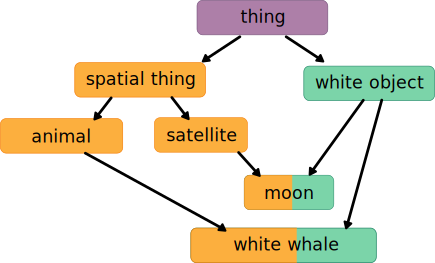
\includegraphics[width=0.7\columnwidth]{oroserver/commonancestors.pdf}
    \caption{Sample taxonomy to illustrate \emph{common ancestors} algorithms.}
    \label{fig|common-ancestors}
\end{figure}

\small
\begin{pseudocode}[ruled]{CommonAncestors}{concept1, concept2}
\label{algo|common-ancestors}

\BEGIN
\mathcal{I} \GETS \CALL{Superclasses}{concept1} \cap \CALL{Superclasses}{concept2} \\
\RETURN {c \in \mathcal{I} | \CALL{Subclasses}{c} \cap \mathcal{I} = \emptyset}\\
\END

\end{pseudocode}
\normalsize

Taking the taxonomy in figure~\ref{fig|common-ancestors} as example, the common
ancestors for the pair \concept{\{white whale, moon\}} are
\concept{\{spatial thing, white object\}}, \ie the set of classes that belong to
the intersection of the super-classes of both the concepts that have no
sub-classes in this intersection.

\small
\begin{pseudocode}[ruled]{FirstDifferentAncestors}{concept1, concept2}
\label{algo|first-different-ancestors}

\BEGIN
\mathcal{C} \GETS \CALL{CommonAncestors}{concept1, concept2} \\
\mathcal{S} \GETS \CALL{Superclasses}{concept1} \cup \CALL{Superclasses}{concept2} \\

\RETURN{\forall c \in \mathcal{C}, \CALL{DirectSubclasses}{c} \cap \mathcal{S}} \\
\END

\end{pseudocode}
\normalsize

The \emph{First Different Ancestors} algorithm
(algorithm~\ref{algo|first-different-ancestors}) returns the list of direct
sub-classes of the common ancestors. They are intuitively the most generic
types that \emph{differenciate} the two concepts. In the taxonomy
figure~\ref{fig|common-ancestors}, two instances \concept{a} and \concept{b} of
respectively \concept{white whale} and \concept{moon} have as first different
ancestors the two sets \concept{\{animal, satellite\}} (subclasses of ancestor
\concept{spatial thing}) and \concept{\{white whale, moon\}} (subclasses of
ancestor \concept{white object}).

\paragraph{Clarification Algorithm}
\label{sect|clarify}

During interactions with other agents, the robot is often required to figure
out which individual correspond to a description like ``red object'', ''a
bottle'', ''a book larger than this other one'', etc. This is a key part of the
grounding capability.

Clarification and discrimination algorithms are based on what we call
\emph{descriptors}: descriptors can be properties of individuals, either
acquired by the robot are statically asserted in a comon-sense ontology. They
are also the result of other reasoning algorithms like the \emph{Common
Ancestors} and \emph{Different Ancestors} algorithms presented above.
We shall see later how symbolic knowledge is first acquired from geometric
reasoning or natural language processing, and we consider in this section that
the \emph{clarification} process is based on an established ontology, like the
sample proposed in figure~\ref{fig|discriminant}.

Based on all this information, and a given partial (or complete) description of
an object (list of attribute-value pairs), the robot is able to identify the
referred object the following way (Algorithm~\ref{algo|clarify}). First it
obtains all objects that fulfill the initial description. Based on the result
it either succeeds (obtains one single object), fails (no object with that
description could be found) or obtains several objects. In this latter case, a
new descriptor is added (mark~\ref{clar.desc}) to the initial description and
the process starts over again until all possible descriptors have been added.

Failure occurs in two cases: when the description does not match any object
from the robot's knowledge, either because the robot's knowledge is incomplete
(the human refers to an unknown descriptor or descriptor value) or due to
inconsistent information (human's and robot's beliefs differ), or when a set of
candidates could not get successfully discriminated with the available
descriptors.

In this latter case, new descriptors new be added (attribute-value pair). Two
alternatives are available: directly asking the human for a new descriptor, or
automatically searching a new attribute and ask the human for its value. In the
latter case, we need to automatically find the best discriminant for the
current list of objects being evaluated ($description$ in the algorithm).


\small
\begin{pseudocode}[ruled]{Clarify}{description}
\label{algo|clarify}
\BEGIN
candidates \GETS \CALL{GetObjectFromDescription}{description} \\
\IF \left|{candidates}\right| = 1 \THEN \RETURN{candidates[0]} \\
\ELSEIF \left|{candidates}\right| = 0 \THEN \OUTPUT{\mbox{No object found!}} \\
\ELSE
    \BEGIN
        description \GETS \CALL{AddDescriptor}{description} \STMTNUM{7em}{clar.desc}\\
        \RETURN{\CALL{Clarify}{description}} \\
    \END
\END

\end{pseudocode}
\normalsize

\paragraph{Finding a discriminant}
\label{sect|discriminant}

\begin{figure}
    \centering
    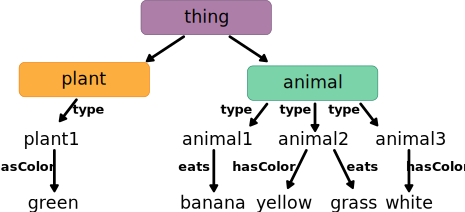
\includegraphics[width=0.7\columnwidth]{oroserver/discriminant.pdf}
    \caption{Sample ontology to illustrate the discrimination routines.
    \concept{plant1} is an instance of \concept{Plant} and
    \concept{animal[1-3]} are instances of \concept{Animal}.}
    \label{fig|discriminant}
\end{figure}

We have implemented a set of semantic categorization functions in ORO. One of
them consists in looking for discriminants, \ie descriptors that allow a
maximum discrimination among a set of individuals. In the example above,
considering the attributes \emph{type, color} and \emph{material}, ORO would
return \emph{color} and \emph{material} as discriminants, since their values
are unique for the given set of objects.

We distinguish two types of discriminants. \emph{Complete} discriminants are
those attributes (or properties) that totally discriminate the set of
individuals. In other words, properties whose values can uniquely identify
those individuals. However, they are not always available. First, because two
or more individuals may share the same value, and second, because not all
individuals may share the same properties. Thus, \emph{partial} discriminants
are those that ``better'' split the set of individuals in different subsets
based on some criteria.

The algorithm to determine the type of discriminant available
(Algorithm~\ref{algo|discriminant}) has the following steps (to better follow
it, we base its description on the ontology example illustrated in
figure~\ref{fig|discriminant}. We search a discriminant for the following
individuals: \concept{plant1}, \concept{animal1}, \concept{animal2} and
\concept{animal3}. First we obtain the direct properties for all the
individuals, \ie we do not consider all the hierarchy of properties. In the
example, \concept{plant1} has two superclasses (\concept{Plant} and
\concept{Thing}), but we only take the most direct one (the class
\concept{Plant}). Next, we compute the number of individuals per property
(mark~\ref{disc.nbind}) and the number of different values for that property
(mark~\ref{disc.nbval}). If there is more than one different value for the
property (in other words, if not all individuals have the same value), then we
consider that property as a potential discriminant (mark~\ref{disc.append}).
Finally, we rank (mark~\ref{disc.rank}) the list of potential properties
following two criteria: the number of individual occurrences (\ie the most
individuals are covered by that property, the better) and the values
occurrences (\ie the more distinct values, the better).  The best discriminant
corresponds to the first element of the sorted list. In other words, the class
with higher number of occurrences and more variety in it.  If several
properties are equal, we return all of them.

In our example, the algorithm would return the class name as the partial
discriminant. If we only consider the instances of the class \concept{Animal},
it would return two properties equally discriminant: \concept{hasColor} and
\concept{eats}. It should be noted that this way of proceeding does not respect
the open world assumption. In this case, we believe that the robot should only
reason based on his current knowledge.

\small
\begin{pseudocode}[ruled]{GetDiscriminant}{individuals}
\label{algo|discriminant}
\BEGIN
P \GETS \CALL{Ontology.GetProperties}{individuals} \\
\hat{P} \GETS \emptyset \\
\FOREACH p \in P \DO
    \BEGIN
        n_{ind} \GETS \CALL{NbIndividualsWithProperty}{p} \STMTNUM{7em}{disc.nbind}\\
        n_{val} \GETS \CALL{NbDifferentValues}{p} \STMTNUM{10.9em}{disc.nbval}\\
        \IF n_{val} > 1 \THEN
            \hat{P} \GETS \CALL{Append}{[p,n_{ind},n_{val}]} \STMTNUM{8.8em}{disc.append}\\
    \END \\

\CALL{Rank}{\hat{P}} \STMTNUM{23.6em}{disc.rank}\\
\RETURN{\hat{P}[0][0]} \\
\END

\end{pseudocode}
\normalsize


\subsubsection{Memory}
\label{sect|oroserver-memory}

The ORO server offers a mechanism to mimick simple forms of biological memory.
When new statements are inserted in the knowledge base, a \emph{memory profile}
can be attached to this set.

Three such profiles are predefined: {\tt short term}, {\tt episodic} and {\tt
long term}. They each correspond to a different lifetime for the statements
(respectively 10 seconds, 5 minutes and no time limit). After this duration,
the statements are automatically removed from the knowledge base.

This approach is limited. In particular, \emph{episodic} memory primarly refers
to the semantics of the statements (that is expected to be related to an event)
and not to a specific life duration. We discuss at the end of this work possible
improvements.

\paragraph{Active Concepts} \emph{Short term} memory, however, is used in real
world applications, in particular to implement the idea of \emph{active
concept}: some modules, like our natural language processor (described later
on, at chapter~\ref{chapt|dialogs}), use the {\tt short term} memory profile to
mark for a few seconds important concepts that are currently manipulated by the
robot. For example, if a human asks the robot: ``Give me all red objects'', the
human, the \concept{Give} action, and each red objects that are found are
successively marked as \emph{active concepts} by inserting statements like
\stmt{human type ActiveConcept} in the short-term memory (which can be
considered, in this case, to be a working memory, as distinguished at
section~\ref{sect|memory}).


\subsubsection{Learning by modifying the knowledge structure}

\subsubsection{Fast Concept Lookup}
\label{sect|oroserver-lookup}

Because this operation is frequent, in particular for language processing
application, the ORO server also provides a fast concept lookup mechanism to
search for a concept identifier by its human-friendly name (label) that takes
into account the language configuration.

%%%%%%%%%%%%%%%%%%%%%%%%%%%%%%%%%%%%%%%%%%%%%%%%%%%%%%%%%%%%%%%%%%%%%%%%%%%%%%
%%%%%%%%%%%%%%%%%%%%%%%%%%%%%%%%%%%%%%%%%%%%%%%%%%%%%%%%%%%%%%%%%%%%%%%%%%%%%%
%%%%%%%%%%%%%%%%%%%%%%%%%%%%%%%%%%%%%%%%%%%%%%%%%%%%%%%%%%%%%%%%%%%%%%%%%%%%%%

\section{Knowledge instanciation: the OpenRobots Common-Sense Ontology}

How much knowledge is available? Which content? How big is the knowledge base?

\subsection{Designing the \textsc{OpenRobots} common-sense ontology}
\label{sect|commonsense-design}

\begin{figure}
    \centering
    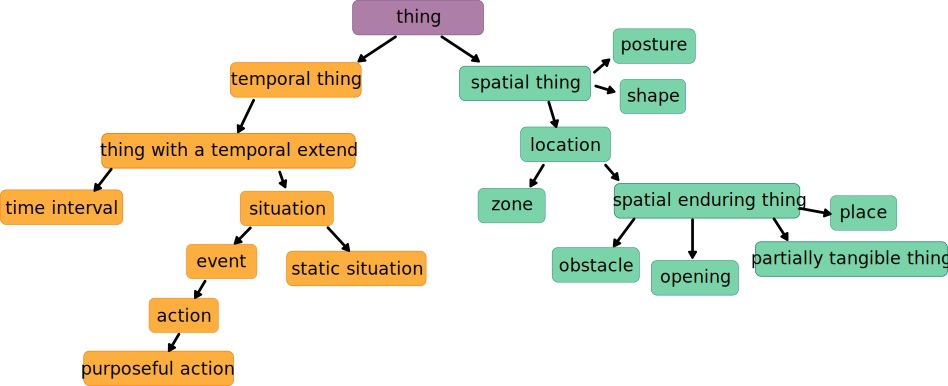
\includegraphics[scale=0.6]{oro/top_tbox.pdf}
    \caption{The upper part of the ORO common-sense TBox.}
    \label{fig|upper_tbox}
\end{figure}

\begin{figure}
    \centering
    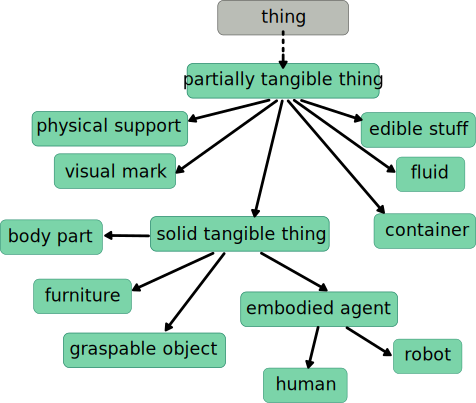
\includegraphics[scale=0.6]{oro/tangible_things_tbox.pdf}
    \caption{TBox of the specializations of \concept{PartiallyTangible}.}
    \label{fig|tangible_things_tbox}
\end{figure}

\subsection{Internationalisation}
\label{sect|commonsense-i13n}
